\chapter{Approach}
\label{cha:approach}

The central idea of the thesis is based on the assumption that humans do their activities in the context of time. Humans follow a certain routine in their lifestyles and time is one de-facto latent element in determination of these routines. Most of the activities in ones daily life can be associated with the time of the day. Thus time is a prominent factor while learning human behaviours and preferences. All the models developed in this thesis try to learn human behaviours and preferences based on time as factor. 

\section{Problem Formulation}
In this thesis we use Bayesian models for representing the learned knowledge about human behaviour and preferences. We formulate the problem as getting an accurate probability density of possible locations given the previous observed locations. Given the corresponding observations of $D_{o_i}$, the probability distribution over the locations of $o_i$ at time $T$ is governed by the following formula 

    \begin{equation} \label{eq:1}
	    P(l_i | t_i, D_{o_i})
    \end{equation}

   Various temporal information related to periodic patterns can be implied by $T$, to indicate the location distribution, such as specific hours of the day (11:00 pm), a day of the week (Friday), or a month of the year (February). We use the \textbf{temporal state} to represent such information and introduce $r(t)$ to denote temporal state extracted from time $T$,.  Dependency on the type of the temporal state $r(t)$ can be a different function. For example, if $r(t)$ denotes temporal state in terms of hours of the day then $r(t) \in {0,1 ... , 23}$, if $r(t)$ denotes temporal state in terms of day of the week, then $r(t) \in {0,1, .. 6}$. Without loss of generality, we use $r(t)$ to denote a type of temporal state in the following description, Equation \ref{eq:1} is reformulated as 
    
    \begin{equation}
	    P( l_i | r(t), D_{o_i})
    \end{equation}
    
    Applying Bayes Rule
    
    \begin{equation}\label{eq:3}
	P( l_i | r(t), D_{o_i}) \propto P(r(t) | l_i, D_{o_i})  P(l_i | D_{o_i})
    \end{equation}
    Where:
    \begin{itemize}[label=]
    \item $P(r(t) | l_i, D_{o_i})$ : Temporal context 
    \item $P(l_i | D_{o_i})$ : Spatial context
    \end{itemize}
    
     The spatial context $P(l_i | D_{o_i})$ indicates the location distribution of object or person $o_i$ given the previous observed location $D_{o_i}$. The temporal context $P(r(t) | l_i, D_{o_i})$ represents the temporal state distribution of object $o_i$, being observed at location $l_i$ with corresponding $D_{o_i}$
    


\begin{tabular}{cp{8cm}}
    \hline
	Symbol & Meaning\\
	\hline
	O & Set of all objects or persons\\
	$o_i$ & Single object from the set $O$, $o_i \in O$ \\
	$L$ & Set of all locations\\
	$l_i$ & Single location from the set $L$. $l_i\in L$\\
    $T$ & Time interval\\
    \hline
	$<o_i,l_i,t_i>$ & object $o_i$ was located at location $l_i$ at time $t_i$\\
	$D$ & Collection of all objects all observed locations\\
	$D_{o_i}$ & Previous observed locations of $o_i$\\ 
    \hline
     $P(r(t) | l_i, D_{o_i})$ &  Temporal context representing the temporal state distribution of $o_i$ at location $l_i$ given previous observations $D_i$\\
     $P(l_i | D_{o_i})$ & Spatial context representing the location distribution of object $o_i$ given the previous observations $D_{o_i}$\\
    \hline
\end{tabular}
% section Problem formulati (end)



\section{Data-Information-Knowledge-Wisdom Hierarchy}

The knowledge generation in the thesis is modelled as a Data-Information-Knowledge-Wisdom (DIKW) Hierarchy\citep{rowley2007wisdom} \citep{ackoff1989data}. \cite{niemueller2012generic} classified the content of the robot mind into this hierarchy and presented a way of knowledge generation using the hierarchy. 
\begin{figure}[htp]
\centering
\includegraphics[width=0.8\textwidth]{images/data-info-knowledge.pdf}
\caption{Knowledge tree for learning user preference in cup positions. Adopted from \citep{niemueller2012generic}}
\label{fig:dikw}
\end{figure}
We use this approach in the knowledge generation of user preferences in our thesis. The approach can be explained using the Figure~\ref{fig:dikw}, where knowledge about the user preference of the cup is generated. The \emph{Data} from different sensors are accessed by the robot. The Data is used to generate \emph{Information} about the location of the cup in the environment. As time progresses more information of the location of the cup are recorded. This recorded informations can then be processed to generate \emph{Knowledge} about the user preferences in cup placement.



\section{Architecture}
\label{cha:}
The overall architecture of learning user preferences can be summarized in the Figure~\ref{fig:architecture}. The robot while, interacting with the environment records all the data (e.g. rgb image ) accumulated by it. Some of the data is used by the robot and converted into useful information (e.g. object location) for completing a particular task. The robot stores this information also in its robot memory. Now periodically or on trigger the robot queries its memory and gathers clusters of information (e.g all the locations of a cup). This queried information is then processed and knowledge is generated from it. This knowledge is again stored back into the robot memory.

\begin{figure}[htp]
\centering
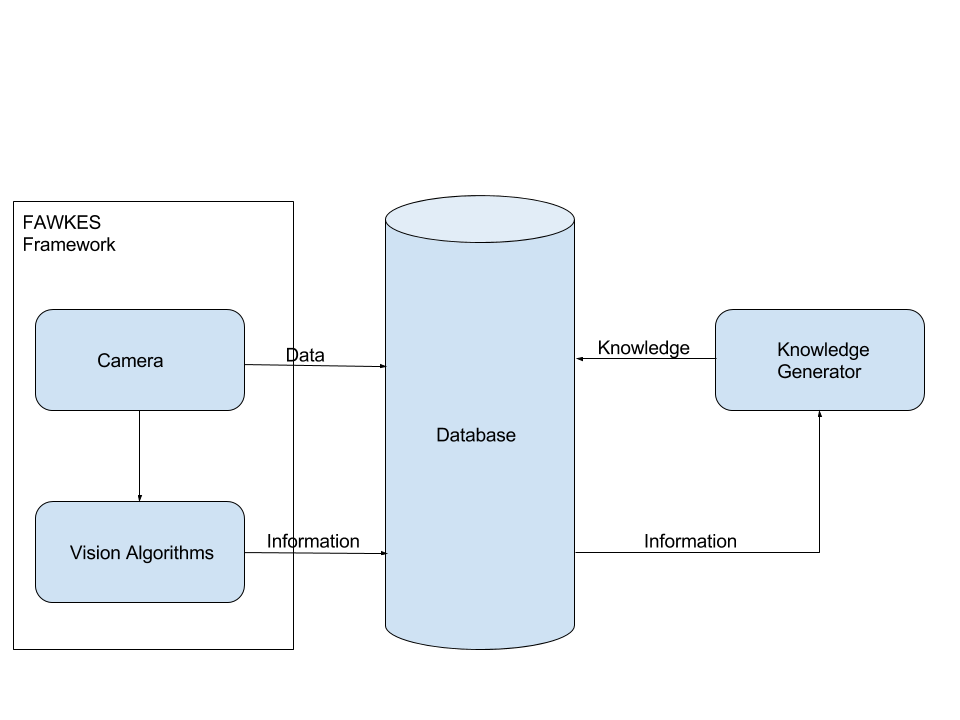
\includegraphics[width=\textwidth]{images/integration.png}
\caption{Integration with the robot memory}
\label{fig:architecture}
\end{figure}


\section{Notation and Terminology}
Throughout the thesis, we are referring to entities such as ``locations," ``hours," and ``observations".
This helps to guide intuition and maintain continuity of thoughts as we go through related problems involving collections of data.
Formally we define the following terms:
\begin{itemize}
	\item A \emph{location} is the basic unit of the discrete data, defined to be an item from a set of locations. These locations can be rooms of the home or different compartments of the kitchen. 
	\item A \emph{period} is a sequence of $N$ locations denoted by $\textbf{p} = {x_1;x_2; \dots ;x_N}$. These represents the locations observed in a particular period of time.
	\item An \emph{observations} is a collection of $T$ periods denoted by $ D = {p_1;p_2; \dots ;p_T}$. These represents the complete data collected by the robot.
\end{itemize}


We also use the entities such as ``data," ``information," and ``knowledge" throughout the thesis \cite{niemueller2012generic}. These can be defined as:
\begin{itemize}
	\item \emph{Data} corresponds to sensor output. All the output of the sensors recorded by the robot is a data. For example, RGB image from a camera, depth points from depth sensors etc.
	\item \emph{Information} corresponds to output of algorithms which process on the above data. For example vision algorithms process RGB images data to extract information of objects or persons in the image.
	\item \emph{Knowledge} corresponds to output of algorithms which process on the above information. For example vision algorithms can process detected object information in consecutive RGB frames to extract knowledge that the object was moving.
\end{itemize}

% section  Things to study (end)